\documentclass[11pt]{article}
\usepackage{geometry}                
\geometry{letterpaper} 
\usepackage{graphicx}
\usepackage{amssymb}
\usepackage{amsmath}
\usepackage{verbatim}
\usepackage{epstopdf}
\usepackage{times}
\usepackage{tikz}
\usetikzlibrary{arrows,automata}

\tikzset{
  treenode/.style = {align=center, inner sep=0pt, text centered,
    font=\sffamily},
  arn_n/.style = {treenode, circle, draw=black,
    , text width=1.5em},% arbre rouge noir, noeud noir
  arn_r/.style = {treenode, circle, red, draw=red, 
    text width=1.5em, very thick},% arbre rouge noir, noeud rouge
   arn_g/.style = {treenode, circle, green, draw=green, 
    text width=1.5em, very thick},% arbre rouge noir, noeud rouge
  arn_x/.style = {treenode, rectangle, draw=black,
    minimum width=0.5em, minimum height=0.5em}% arbre rouge noir, nil
}

\DeclareGraphicsRule{.tif}{png}{.png}{`convert #1 `dirname #1`/`basename #1 .tif`.png}

\title{CS181 - Homework 1}
\author{Lucas Freitas and Angela Li}
\date{\today}

\begin{document}

\maketitle
\begin {enumerate}
%NUMBER 1
\item
\begin {enumerate}
\item
\begin{enumerate}
\item
For $A$:
\newline
\newline
$H(label)$: $\#(yes)=4$, $\#(no)=3$, so:
$$p(yes)=\frac{4}{7}$$
$$p(no)=\frac{3}{7}$$
$$H(label)=\frac{4}{7}log_2(\frac{7}{4})+\frac{3}{7}log_2(\frac{7}{3})\approx0.985$$

$H(label|A=true)=1$, since it is equally likely to be positive or negative given that $A=true$.
\newline

$H(label|A=false)$: $\#(yes)=2$, $\#(no)=1$, so:
$$p(yes)=\frac{2}{3}$$
$$p(no)=\frac{1}{3}$$
$$H(label|A=false)=\frac{2}{3}log_2(\frac{3}{2})+\frac{1}{3}log_2(3)\approx0.918$$

Therefore:
$$H(label|A)=p(A=true)H(label|A=true)+p(A=false)H(label|A=false)$$
$$H(label|A)=\frac{4}{7}H(label|A=true)+\frac{3}{7}H(label|A=false)\approx 0.965$$

Finally:
$$I(label; A)=H(label)-H(label|A)\approx0.02$$

\item
For $B$:
\newline
\newline
$H(label|B=true)=1$, since it is equally likely to be positive or negative given that $B=true$.
\newline

$H(label|B=false)$: $\#(yes)=3$, $\#(no)=2$, so:
$$p(yes)=\frac{3}{5}$$
$$p(no)=\frac{2}{5}$$
$$H(label|B=false)=\frac{3}{5}log_2(\frac{5}{3})+\frac{2}{5}log_2(\frac{5}{2})\approx0.971$$

Therefore:
$$H(label|B)=p(B=true)H(label|B=true)+p(B=false)H(label|B=false)$$
$$H(label|A)=\frac{2}{7}H(label|A=true)+\frac{5}{7}H(label|A=false)\approx 0.979$$

Finally:
$$I(label; B)=H(label)-H(label|B)\approx0.006$$

\end{enumerate}
Thus, ID3 would split on $A$, since that gives a higher information gain. An argument in favor of splitting on A is that it is a more "extreme" split with more disparate probabilities, meaning it will more resolutely divide the data. An argument in favor of splitting on B is that it will classify a larger subset well.
\\ \\
This shows that the inductive bias of ID3 is to prefer more "extreme" splits which more resolutely divide the data. 

\item
From looking at the data it is fairly obvious that in figuring out the first attribute to split on, B, C, and D have the same information gain. Since we calculated that A has a higher information gain than B, we'll first split on A. When A is 1, we can split on either B or C, which still have the same information gain at this step; we can recurse in a similar fashion from there, preferring binary splits. When A is 0, we can again split on either B or C, but (assuming we pick B) we run into the base case of no more information gain after traveling down the 0 path. So we can set that leaf to the most common label, 1.

\begin{center}
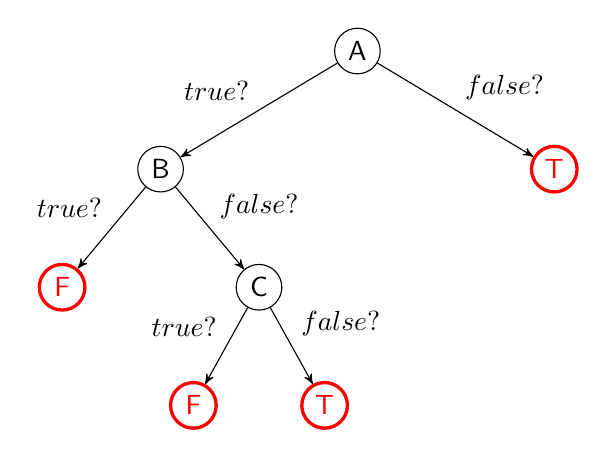
\begin{tikzpicture}[->,>=stealth',level/.style={sibling distance = 5cm/#1,
  level distance = 1.5cm}] 
\node [arn_n] {A} 
    child{ node [arn_n] {B} 
            child{ node [arn_r] {F} edge from parent node[above left]
                         {$true?$}} %for a named pointer
            child{ node [arn_n] {C}   
							child{ node [arn_r] {F} edge from parent node[above left]
                         {$true?$}} 
							child{ node [arn_r] {T} edge from parent node[above right]
                         {$false?$}} edge from parent node[above right]
                         {$false?$}
            }   edge from parent node[above left]
                         {$true?$}                         
    }
    child{ node [arn_r] {T} edge from parent node[above right]
                         {$false?$}} %for a named pointer
; 
\end{tikzpicture}
\end{center}


\item %% INSERT TREE hERE %% 
This tree has a training error of 1/7, just like the ID3 tree produced above. It shows us that ID3 certainly does not always generate the shortest trees, and specifically that preferring higher information gain for individual attributes at a time (and not being able to look ahead at combinations of attributes) often does not produce the most concise tree.

\begin{center}
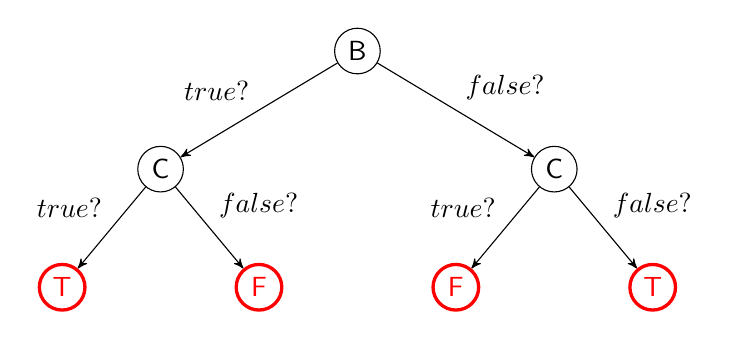
\begin{tikzpicture}[->,>=stealth',level/.style={sibling distance = 5cm/#1,
  level distance = 1.5cm}] 
\node [arn_n] {B} 
    child{ node [arn_n] {C} 
            child{ node [arn_r] {T} edge from parent node[above left]
                         {$true?$}} %for a named pointer
            child{ node [arn_r] {F}  edge from parent node[above right]
                       {$false?$}} %for a named pointer
    edge from parent node[above left]
                       {$true?$} %for a named pointer
    }
    child{ node [arn_n] {C} 
                     child{ node [arn_r] {F} edge from parent node[above left]
                         {$true?$}} %for a named pointer
            child{ node [arn_r] {T}  edge from parent node[above right]
                       {$false?$}} %for a named pointer
    edge from parent node[above right]
                       {$false?$} %for a named pointer    
                     } %for a named pointer
; 
\end{tikzpicture}
\end{center}

\end{enumerate}

%NUMBER 2
\item
\begin{enumerate}
\item
The average cross-validated training and test performance over the ten trials for the non-noisy dataset is $0.87$ and $0.78$ for the noisy dataset.

\item
\begin{enumerate}
\item
Graphs outputted from the Python script:

\begin{verbatim}
$ python main.py
\end{verbatim}



\item
\begin{enumerate}
\item
For non-noisy data: the performance of the train data initially oscillates, but then increases almost monotonically, reaching $100\%$ performance when the validation set size reaches $78$. The test data performance oscillates a lot, reaching a maximum at validation set size $21$, with performance $ 89\%$, which is slightly higher ($\approx2.3\%$ increase) than the one obtained without pruning. The performance then decreases, reaching $76\%$ performance for a validation set of size $80$.

\item
For noisy data: the performance of the train data initially oscillates, but then also increases almost monotonically, reaching $\approx98.3\%$ performance when the validation set size reaches $78$. The test data performance oscillates a lot, reaching a maximum at validation set size $8$, with performance $82\%$, which is slightly higher ($\approx5.1\%$ increase) than the one obtained without pruning. The performance then decreases, reaching $71\%$ performance for a validation set of size $80$.
\end{enumerate}

\item
For some values of the validation set, yes. As mentioned in the previous item, for the non-noisy data we reach an $89\%$ performance at validation set size $21$, which is a $\approx2.3\%$ increase in the performance of ID3, while for noisy data the maximum occurs at validation set size $8$ with $82\%$ performance, which is a $\approx5.1\%$ increase) in the performance of ID3. If the validation set is too large, however, the ID3 performance decreases ($\approx12.6\%$ performance decrease for non-noisy and $8.97\%$ for noisy).
\item

\end{enumerate}

\end{enumerate}

%NUMBER 3
\item

%NUMBER 4
\item

\begin{center}
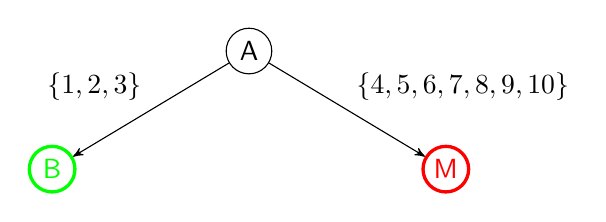
\begin{tikzpicture}[->,>=stealth',level/.style={sibling distance = 5cm/#1,
  level distance = 1.5cm}] 
\node [arn_n] {A} 
    child{ node [arn_g] {B}edge from parent node[above left] {$\{1,2,3\}$} }
    child{ node [arn_r] {M} edge from parent node[above right] {$\{4,5,6,7,8,9,10\}$} }
   ; 
\end{tikzpicture}
\end{center}



\end{enumerate}
\end{document}  